% Fig 1 — IRexp positioning among spectral resources.
% Honest log-scale lollipop chart with dual (position + size) magnitude encoding,
% access-type tags (view-only / open-access / this work) and a redistribution callout.
\documentclass[border=0pt,tikz]{standalone}
% Nature Portfolio / Scientific Data shared TikZ style for IRexp figures.
% Width: 183 mm double-column. Typography: Helvetica-class (phv).
\RequirePackage{tikz}
\RequirePackage{pgfplots}
\RequirePackage{xcolor}
\RequirePackage{helvet}
\IfFileExists{sansmathfonts.sty}{\RequirePackage{sansmathfonts}}{}
\renewcommand{\familydefault}{\sfdefault}
\pgfplotsset{compat=1.18}
\usetikzlibrary{
  arrows.meta,calc,positioning,fit,shapes.geometric,shapes.misc,
  backgrounds,shadows.blur,patterns,decorations.pathreplacing
}

% ---- Paul Tol / NMRexp-matched palette ----
\definecolor{nmrBlue}{HTML}{4A7EBB}
\definecolor{nmrBlueDark}{HTML}{2E5F8F}
\definecolor{nmrBlueLight}{HTML}{A8C8E8}
\definecolor{nmrPeach}{HTML}{E8B48C}
\definecolor{nmrNavy}{HTML}{1B3D5C}
\definecolor{nmrRed}{HTML}{C44E52}
\definecolor{nmrGreen}{HTML}{3D8B5E}
\definecolor{nmrOrange}{HTML}{D97B32}
\definecolor{ink}{HTML}{1A1A1A}
\definecolor{muted}{HTML}{7A7F85}
\definecolor{note}{HTML}{5C636A}
\definecolor{faint}{HTML}{E8EAEC}
\definecolor{ghost}{HTML}{C5C9CD}
\definecolor{tintBlue}{HTML}{EEF3F8}
\definecolor{tintGreen}{HTML}{EAF4EE}

\newcommand{\NatureFont}{\fontfamily{phv}\selectfont}
\newcommand{\PanelLabel}[1]{%
  {\NatureFont\bfseries\fontsize{8}{9.6}\selectfont #1}%
}
\newcommand{\FigBody}{\NatureFont\fontsize{7}{8.4}\selectfont}
\newcommand{\FigSmall}{\NatureFont\fontsize{5.5}{6.6}\selectfont}
\newcommand{\FigAxis}{\NatureFont\fontsize{7}{8.4}\selectfont}

\tikzset{
  nature arrow/.style={
    -{Latex[length=1.6mm,width=1.3mm]},
    line width=0.55pt, ink
  },
  nature arrow grey/.style={
    -{Latex[length=1.6mm,width=1.3mm]},
    line width=0.5pt, note
  },
  stage card/.style={
    draw=nmrBlueDark, line width=0.7pt, rounded corners=2.2pt,
    fill=white, inner sep=3pt, align=center, font=\FigBody
  },
  stage header/.style={
    fill=nmrBlueDark, text=white, font=\FigBody\bfseries,
    rounded corners=2.2pt, inner sep=2.5pt, align=center
  },
  soft card/.style={
    draw=ghost, line width=0.55pt, rounded corners=2.2pt,
    fill=white, inner sep=3.5pt, align=left, font=\FigBody
  },
}

\pgfplotsset{
  nature axis/.style={
    tick label style={font=\FigSmall, /pgf/number format/assume math mode},
    label style={font=\FigAxis\bfseries},
    title style={font=\FigBody\bfseries, color=ink},
    axis line style={ink, line width=0.5pt},
    tick style={ink, line width=0.45pt},
    major grid style={faint, line width=0.35pt},
    axis x line=bottom,
    axis y line=left,
    enlarge x limits=false,
    clip=false,
  },
  nature hbar/.style={
    nature axis,
    xbar,
    bar width=7pt,
    y=data,
    nodes near coords,
    every node near coord/.append style={
      font=\FigSmall, ink, anchor=west, /pgf/number format/fixed,
      /pgf/number format/1000 sep={,}
    },
    xtick=\empty,
    axis x line=none,
    y axis line style={ink, line width=0.55pt},
    ytick style={draw=none},
    y tick label style={font=\FigBody, ink, anchor=east},
    grid=major x,
    xmin=0,
  },
}


\begin{document}
\NatureFont
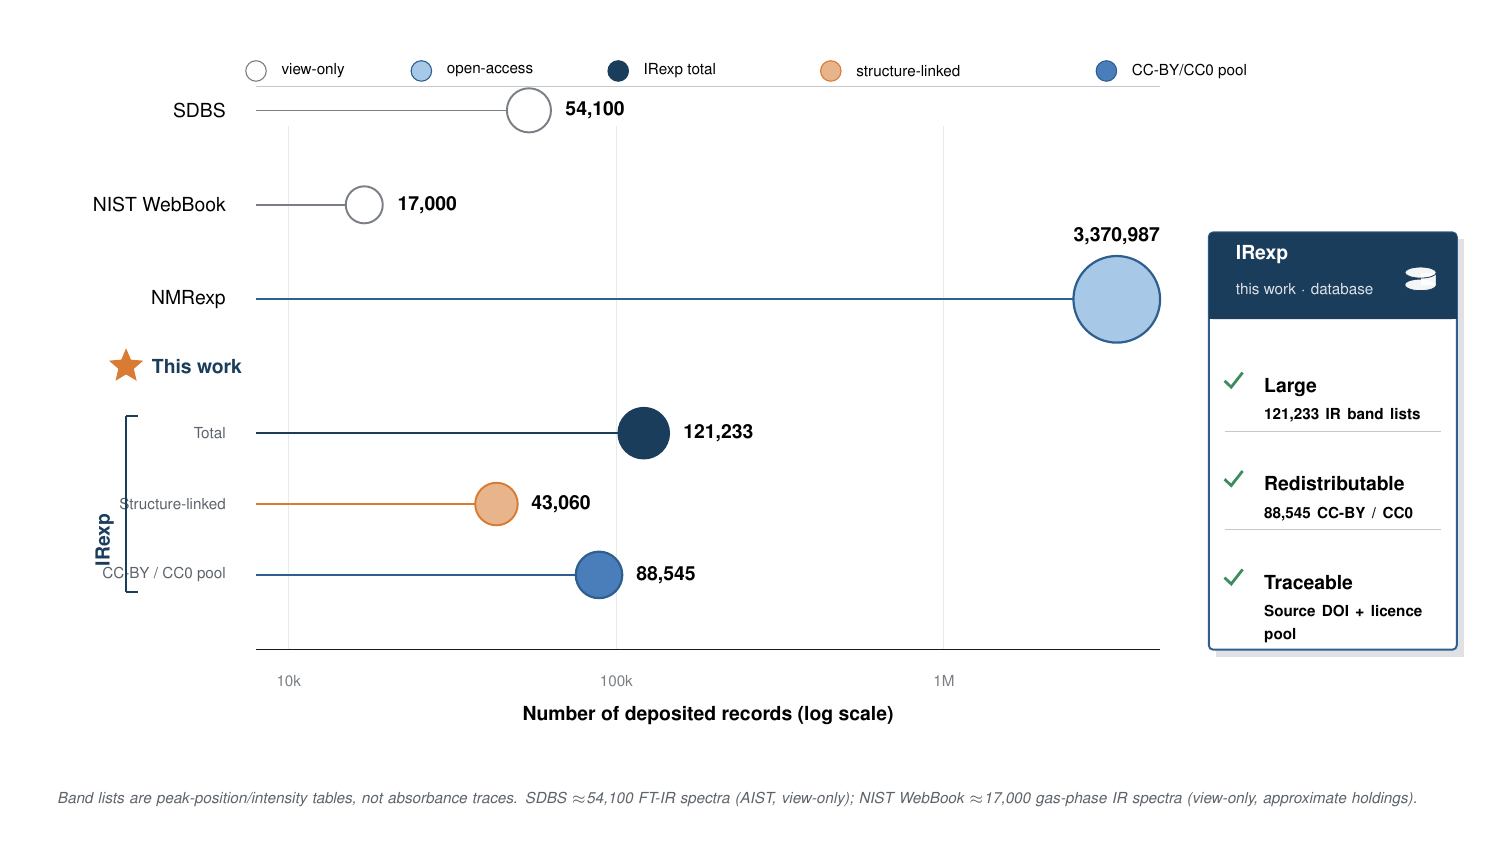
\begin{tikzpicture}[x=1mm,y=1mm]

% ---------------------------------------------------------------------------
% Geometry
% ---------------------------------------------------------------------------
\pgfmathsetmacro{\xmin}{3.9}      % log10(value) lower bound
\pgfmathsetmacro{\xmax}{6.66}     % log10(value) upper bound
\pgfmathsetmacro{\DecScale}{41.6} % mm per decade
\pgfmathsetmacro{\XO}{29}         % plot origin (x, mm) on canvas
\pgfmathsetmacro{\YO}{22}         % axis baseline (y, mm) on canvas

% NB: pgfmath's ln()/exp() route through TeX dimensions internally, which
% overflow ("Dimension too large") for raw values above a few thousand.
% We therefore take log10 of the value expressed in THOUSANDS (+3 decades).
\pgfmathsetmacro{\xSDBS}{((ln(54.100)/ln(10)+3)-\xmin)*\DecScale}
\pgfmathsetmacro{\xNIST}{((ln(17.000)/ln(10)+3)-\xmin)*\DecScale}
\pgfmathsetmacro{\xNMR}{((ln(3370.987)/ln(10)+3)-\xmin)*\DecScale}
\pgfmathsetmacro{\xTot}{((ln(121.233)/ln(10)+3)-\xmin)*\DecScale}
\pgfmathsetmacro{\xStruct}{((ln(43.060)/ln(10)+3)-\xmin)*\DecScale}
\pgfmathsetmacro{\xCC}{((ln(88.545)/ln(10)+3)-\xmin)*\DecScale}
\pgfmathsetmacro{\xgA}{((ln(10)/ln(10)+3)-\xmin)*\DecScale}
\pgfmathsetmacro{\xgB}{((ln(100)/ln(10)+3)-\xmin)*\DecScale}
\pgfmathsetmacro{\xgC}{((ln(1000)/ln(10)+3)-\xmin)*\DecScale}
\pgfmathsetmacro{\PW}{(\xmax-\xmin)*\DecScale} % plot width

% row y-positions (mm above axis baseline)
\def\ySDBS{68.5}
\def\yNIST{56.5}
\def\yNMR{44.5}
\def\yTot{27.5}
\def\yStruct{18.5}
\def\yCC{9.5}

% ---------------------------------------------------------------------------
% Canvas frame (invisible, fixes bounding box at 183 x 101 mm)
% ---------------------------------------------------------------------------
\useasboundingbox (0,0) rectangle (183,101);

% ---------------------------------------------------------------------------
% Plot background: minor decade grid
% ---------------------------------------------------------------------------
\begin{scope}[shift={(\XO,\YO)}]
  \foreach \gx/\glab in {\xgA/{10k},\xgB/{100k},\xgC/{1M}}{
    \draw[faint, line width=0.4pt] (\gx,0) -- (\gx,66.5);
    \node[font=\FigSmall,text=muted,anchor=north] at (\gx,-2.0) {\glab};
  }
  \draw[ink, line width=0.5pt] (0,0) -- (\PW,0); % baseline
\end{scope}

% x-axis title (below tick labels, clear of footnote)
\node[font=\FigAxis,anchor=north,align=center] at (\XO+\PW/2,\YO-6.0)
  {\bfseries Number of deposited records (log scale)};

% ---------------------------------------------------------------------------
% Access-type legend row (top)
% ---------------------------------------------------------------------------
\begin{scope}[shift={(\XO,0)}]
  \def\legY{95.5}
  \node[circle,draw=muted,fill=white,minimum size=2.6mm,inner sep=0] at (0,\legY) {};
  \node[font=\FigSmall,anchor=west] at (2,\legY) {view-only};
  \node[circle,draw=nmrBlueDark,fill=nmrBlueLight,minimum size=2.6mm,inner sep=0] at (21,\legY) {};
  \node[font=\FigSmall,anchor=west] at (23,\legY) {open-access};
  \node[circle,draw=nmrNavy,fill=nmrNavy,minimum size=2.6mm,inner sep=0] at (46,\legY) {};
  \node[font=\FigSmall,anchor=west] at (48,\legY) {IRexp total};
  \node[circle,draw=nmrOrange,fill=nmrPeach,minimum size=2.6mm,inner sep=0] at (73,\legY) {};
  \node[font=\FigSmall,anchor=west] at (75,\legY) {structure-linked};
  \node[circle,draw=nmrBlueDark,fill=nmrBlue,minimum size=2.6mm,inner sep=0] at (108,\legY) {};
  \node[font=\FigSmall,anchor=west] at (110,\legY) {CC-BY/CC0 pool};
\end{scope}
\draw[ghost,line width=0.4pt] (\XO,93.5) -- (\XO+\PW,93.5);

% ---------------------------------------------------------------------------
% Lollipops — comparators (SDBS, NIST, NMRexp)
% ---------------------------------------------------------------------------
\begin{scope}[shift={(\XO,\YO)}]
  % leader lines
  \draw[muted, line width=0.6pt] (0,\ySDBS) -- (\xSDBS,\ySDBS);
  \draw[muted, line width=0.6pt] (0,\yNIST) -- (\xNIST,\yNIST);
  \draw[nmrBlueDark, line width=0.7pt] (0,\yNMR) -- (\xNMR,\yNMR);

  % markers (size ~ log magnitude)
  \node[circle,draw=muted,line width=0.7pt,fill=white,minimum size=5.6mm,inner sep=0] at (\xSDBS,\ySDBS) {};
  \node[circle,draw=muted,line width=0.7pt,fill=white,minimum size=4.7mm,inner sep=0] at (\xNIST,\yNIST) {};
  \node[circle,draw=nmrBlueDark,line width=0.8pt,fill=nmrBlueLight,minimum size=11mm,inner sep=0] (nmrDot) at (\xNMR,\yNMR) {};

  % value labels
  \node[font=\FigBody,anchor=west] at (\xSDBS+3.4,\ySDBS) {\bfseries 54,100};
  \node[font=\FigBody,anchor=west] at (\xNIST+3.0,\yNIST) {\bfseries 17,000};
  \node[font=\FigBody,anchor=south] at (nmrDot.north) {\bfseries 3,370,987};

  % row category labels (left of axis)
  \node[font=\FigBody,anchor=east] at (-2.6,\ySDBS) {SDBS};
  \node[font=\FigBody,anchor=east] at (-2.6,\yNIST) {NIST WebBook};
  \node[font=\FigBody,anchor=east] at (-2.6,\yNMR) {NMRexp};
\end{scope}

% ---------------------------------------------------------------------------
% IRexp group (Total / Structure-linked / CC-BY,CC0) with bracket + star badge
% ---------------------------------------------------------------------------
\begin{scope}[shift={(\XO,\YO)}]
  \draw[nmrNavy, line width=0.9pt] (0,\yTot) -- (\xTot,\yTot);
  \draw[nmrOrange, line width=0.8pt] (0,\yStruct) -- (\xStruct,\yStruct);
  \draw[nmrBlueDark, line width=0.8pt] (0,\yCC) -- (\xCC,\yCC);

  \node[circle,draw=nmrNavy,line width=0.8pt,fill=nmrNavy,minimum size=6.4mm,inner sep=0] at (\xTot,\yTot) {};
  \node[circle,draw=nmrOrange,line width=0.7pt,fill=nmrPeach,minimum size=5.4mm,inner sep=0] at (\xStruct,\yStruct) {};
  \node[circle,draw=nmrBlueDark,line width=0.8pt,fill=nmrBlue,minimum size=5.9mm,inner sep=0] at (\xCC,\yCC) {};

  \node[font=\FigBody,anchor=west] at (\xTot+3.8,\yTot) {\bfseries 121,233};
  \node[font=\FigBody,anchor=west] at (\xStruct+3.2,\yStruct) {\bfseries 43,060};
  \node[font=\FigBody,anchor=west] at (\xCC+3.5,\yCC) {\bfseries 88,545};

  \node[font=\FigSmall,anchor=east,text=note] at (-2.6,\yTot) {Total};
  \node[font=\FigSmall,anchor=east,text=note] at (-2.6,\yStruct) {Structure-linked};
  \node[font=\FigSmall,anchor=east,text=note] at (-2.6,\yCC) {CC-BY / CC0 pool};

  % bracket + group label
  \draw[nmrNavy,line width=0.8pt] (-16.5,\yTot+2.2) -- (-16.5,\yCC-2.2);
  \draw[nmrNavy,line width=0.8pt] (-16.5,\yTot+2.2) -- (-15.0,\yTot+2.2);
  \draw[nmrNavy,line width=0.8pt] (-16.5,\yCC-2.2) -- (-15.0,\yCC-2.2);
  \node[font=\FigBody,anchor=east,rotate=90,text=nmrNavy] at (-19.2,\yStruct) {\bfseries IRexp};

  % "This work" star badge, anchored to the group bracket
  \node[star,star points=5,star point ratio=2.2,fill=nmrOrange,draw=nmrOrange,
        minimum size=4.2mm,inner sep=0] (star) at (-16.5,\yTot+8.5) {};
  \node[font=\FigBody,anchor=west,text=nmrNavy] at (star.east) {\bfseries\;This work};
\end{scope}

% ---------------------------------------------------------------------------
% Sidebar callout card
% ---------------------------------------------------------------------------
\def\SBx{150.0}
\def\SBy{\YO}
\def\SBw{31.5}
\def\SBh{53.0}
\def\SBtxw{23mm}

% soft offset shadow
\fill[ghost,opacity=0.55]
  ($(\SBx,\SBy)+(0.9,-0.9)$) rectangle ($(\SBx+\SBw,\SBy+\SBh)+(0.9,-0.9)$);
% card
\draw[draw=nmrBlueDark,line width=0.7pt,fill=white,rounded corners=1.6pt]
  (\SBx,\SBy) rectangle (\SBx+\SBw,\SBy+\SBh);
% header
\fill[nmrNavy,rounded corners=1.6pt] (\SBx,\SBy+\SBh-11.0) rectangle (\SBx+\SBw,\SBy+\SBh);
\fill[nmrNavy] (\SBx,\SBy+\SBh-11.0) rectangle (\SBx+\SBw,\SBy+\SBh-5.5);
\node[font=\FigBody,anchor=west,text=white] at (\SBx+2.2,\SBy+\SBh-2.8) {\bfseries IRexp};
\node[font=\FigSmall,anchor=west,text=white!85!nmrNavy] at (\SBx+2.2,\SBy+\SBh-7.2) {this work $\cdot$ database};

% mini DB-cylinder icon (top-right corner of header, clear of text)
\begin{scope}[shift={(\SBx+\SBw-4.6,\SBy+\SBh-5.5)}]
  \fill[white,opacity=0.95] (0,-1.2) rectangle (2.0,0.4);
  \fill[white,opacity=0.95] (0,0.4) ellipse (2.0mm and 0.7mm);
  \fill[white,opacity=0.95] (0,-1.2) ellipse (2.0mm and 0.7mm);
  \draw[nmrNavy,line width=0.3pt] (0,0.4) ellipse (2.0mm and 0.7mm);
  \draw[nmrNavy,line width=0.3pt] (-2.0,0.4) -- (-2.0,-1.2) arc (180:360:2.0mm and 0.7mm) -- (2.0,0.4);
\end{scope}

% checkmark bullets
\newcommand{\Check}[3]{%
  \draw[nmrGreen,line width=1.0pt] (#1,#2+0.15) -- (#1+0.85,#2-0.65) -- (#1+2.3,#2+1.2);
  \node[font=\FigBody,anchor=north west,align=left,text width=\SBtxw] at (#1+3.8,#2+1.7) {#3};
}
\Check{\SBx+2.0}{\SBy+34.0}{\bfseries Large\\[1.5pt]{\FigSmall 121,233 IR band lists}}
\Check{\SBx+2.0}{\SBy+21.5}{\bfseries Redistributable\\[1.5pt]{\FigSmall 88,545 CC-BY / CC0}}
\Check{\SBx+2.0}{\SBy+9.0}{\bfseries Traceable\\[1.5pt]{\FigSmall Source DOI + licence pool}}

\draw[ghost,line width=0.4pt] (\SBx+2.0,\SBy+27.75) -- (\SBx+\SBw-2.0,\SBy+27.75);
\draw[ghost,line width=0.4pt] (\SBx+2.0,\SBy+15.25) -- (\SBx+\SBw-2.0,\SBy+15.25);

% ---------------------------------------------------------------------------
% Footnote (bottom, honesty rule)
% ---------------------------------------------------------------------------
\node[font=\FigSmall,anchor=south west,text=note,align=left,text width=178mm] at (2.5,0.8)
 {\itshape Band lists are peak-position/intensity tables, not absorbance traces. SDBS $\approx$54,100 FT-IR spectra (AIST, view-only); NIST WebBook $\approx$17,000 gas-phase IR spectra (view-only, approximate holdings).};

\end{tikzpicture}
\end{document}
